\documentclass{article}
\usepackage[utf8]{inputenc}
\usepackage{graphicx}
	\DeclareGraphicsExtensions{.png, .jpeg}
\usepackage{caption}
% \usepackage{subcaption}
\usepackage{csvsimple}
\usepackage[top=1in, bottom=1in, left=1in, right=1in]{geometry}

\title{Database Design and Implementation \\ HW 03}
\author{\underline{Team 08}\\Henriod, Terence\\Santoyo, Jorge \\Singh, Raja}
\date{\today}

\begin{document}

\clearpage
\maketitle
\thispagestyle{empty} % removes the page number from the title page

\begin{abstract}
An introductory assignment to become familiarized with creating and populating database tables using SQL.
\end{abstract}

\newpage
\section{Assignment Background}
The purpose of this assignment is to create tables with constraints and then populate those tables with data to produce a test database for CutGlass Mosaic \& Tile, a hard surface (tile, glass, marble, granite, etc.) subcontracting firm. CutGlass provides hard surface removal, design, installation, and maintenance services.  The company creates complex, artistic mosaics as well as simple, standard tile floors.  CutGlass employs a range of workers including artistic designers, surface removal specialists, and tiling craftsmen.\\\\
The application for this assignment is part of their job costing system.  The purpose of the database is to collect actual labor and material costs and assign those costs to a specific task on a specific job.  The job costing system is used to compare actual direct costs for labor and materials to estimated costs for labor and materials by task on a job.  In addition, this system will be used to compare actual labor hours to estimated labor hours.  Thus, employee hours are also assigned to a task on a job.\\\\
Your objective for this assignment is to create ten tables in your existing database as described in this document and populate those tables with the data included on the pages following the table descriptions.  Please do not make up different data – you must use the data included in this document.  I want everyone in class to be working from exactly the same test dataset.\\\\
This assignment is not especially difficult, but it may be time-consuming. It is a good way to become familiar with SQL syntax and Microsoft’s SQL Server, so bear with it - the next three assignments build on this one and are more challenging and fun!\\

\begin{figure}[h]
  \centering
  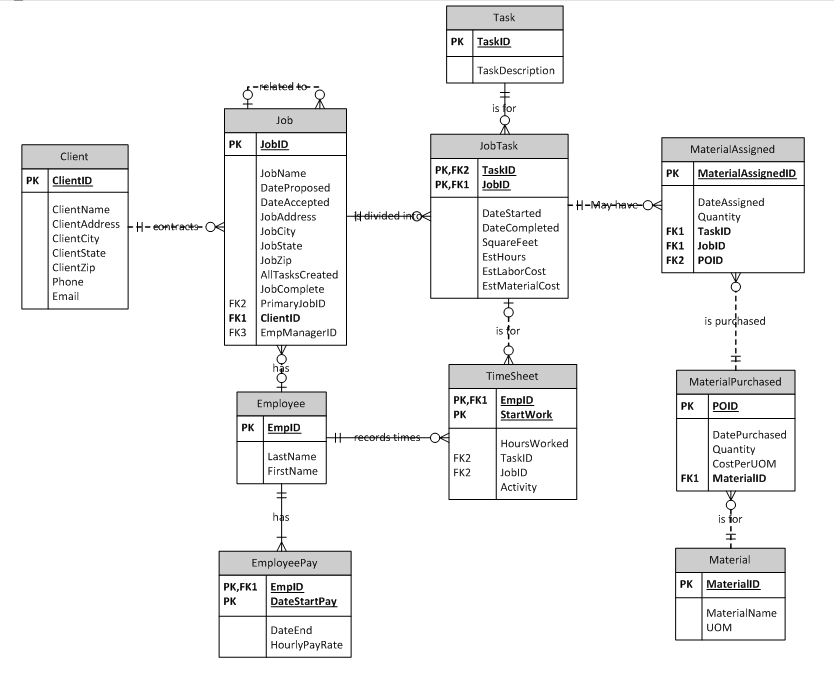
\includegraphics[width=.8\linewidth]{HW03_ERD}
  \caption{The solution ERD for Chemical Engineering Company's database.}
  \label{fig:ERD}
\end{figure}

\section{Creating Tables}
Give the \texttt{CREATE TABLE} statements used to create each of the tables.\\

\textit{Solution}:
\begin{verbatim}
    CREATE TABLE Client(
        ClientID int NOT NULL,
        ClientName varchar(30) NOT NULL,
        ClientAddress varchar(30) NOT NULL,
        ClientCity varchar(15) NOT NULL,
        ClientState char(32) NOT NULL,
        ClientZip varchar(12) NOT NULL,
        Phone char(10) NOT NULL,
        Email varchar(50),
        CONSTRAINT pk_ClientID PRIMARY KEY(ClientID)
    );

    CREATE TABLE Employee(
        EmpID int NOT NULL,
        LastName varchar(30) NOT NULL,
        FirstName varchar(30),
        CONSTRAINT pk_EmpID PRIMARY KEY(EmpID) 
    );

    CREATE TABLE Task(
        TaskID int NOT NULL,
        TaskDescription varchar(50) NOT NULL,
        CONSTRAINT pk_TaskID PRIMARY KEY(TaskID)
    );

    CREATE TABLE Job(
        JobID int NOT NULL,
        JobName varchar(40) NOT NULL,
        DateProposed Date NOT NULL,
        DateAccepted Date,
        JobAddress varchar(30),
        JobCity varchar(15),
        JobState char(2),
        JobZip varchar(12),
        AllTaskCreated Bit NOT NULL, 
        JobCompleted Bit NOT NULL,
        PrimaryJobID int,
        ClientID int NOT NULL,
        EmpManagerID int, 
        CONSTRAINT pk_JobID PRIMARY KEY(JobID),
        CONSTRAINT fk_PrimaryJobID FOREIGN KEY (PrimaryJobID) REFERENCES Job(JobID),
        CONSTRAINT fk_ClientID FOREIGN KEY (ClientID) REFERENCES Client(ClientID),
        CONSTRAINT fk_EmpManagerID FOREIGN KEY (EmpManagerID) REFERENCES Employee(EmpID)
    );

    CREATE TABLE JobTask(
        TaskID int NOT NULL,
        JobID int NOT NULL,
        DateStarted Date NOT NULL,
        DateCompleted Date,
        SquareFeet int NOT NULL,
        EstHours int NOT NULL,
        EstLaborCost Money NOT NULL,
        EstMaterialCost Money NOT NULL,
        CONSTRAINT pk_JobTask PRIMARY KEY(TaskID,JobID),
        CONSTRAINT fk_TaskID FOREIGN KEY(TaskID) REFERENCES Task(TaskID),
        CONSTRAINT fk_JobID FOREIGN KEY(JobID) REFERENCES Job(JobID)
    );

    CREATE TABLE EmployeePay(
        EmpID int NOT NULL,
        DateStartPay Date NOT NULL,
        DateEnd Date,
        HourlyPayRate Money NOT NULL,
        CONSTRAINT pk_employeePay PRIMARY KEY (EmpID,DateStartPay),
        CONSTRAINT fk_EmpID FOREIGN KEY (EmpID) REFERENCES Employee(EmpID) 
    );

    CREATE TABLE TimeSheet(
        EmpID int NOT NULL,
        StartWork DateTime NOT NULL,
        HoursWorked Decimal (4,2) NOT NULL,
        TaskID int,
        JobID int,
        Activity varchar(15),
        CONSTRAINT pk_TImeSheet PRIMARY KEY(EmpID,StartWork),
        CONSTRAINT fk_TimeSheetEmpID FOREIGN KEY(EmpID) REFERENCES Employee(EmpID),
        CONSTRAINT fk_JobTaskID FOREIGN KEY(TaskID,JobID) REFERENCES JobTask(TaskID,JobID),
    );


    CREATE TABLE Material(
        MaterialID int NOT NULL,
        MaterialName varchar(50) NOt NULL,
        UOM varchar(5),
        CONSTRAINT pk_MaterialID PRIMARY KEY(MaterialID),
        CHECK ( UOM = `Tube' OR  UOM = `SQFT' OR UOM = `Sheet' OR 
                UOM = `qt' OR UOM = `lb' OR UOM = `gal' OR UOM = `ea' OR  UOM = `ft' OR
                UOM =`ton' OR UOM  = `pint' )
    );

    CREATE TABLE MaterialPurchased(
        POID int NOT NULL,
        DatePurchased DateTime NOT NULL,
        Quantity Decimal (7,2) NOT NULL,
        CostPerUOM Money NOT NULL,
        MaterialID int NOT NULL,
        CONSTRAINT pk_POID PRIMARY KEY(POID),
        CONSTRAINT fk_MaterialID FOREIGN KEY(MaterialID) REFERENCES Material(MaterialID)
    );

    CREATE TABLE MaterialAssigned(
        MaterialAssignedID int NOT NULL IDENTITY (1000,1),
        DateAssigned DateTime NOT NULL,
        Quantity Decimal(7,2) NOT NULL,
        TaskID int NOT NULL,
        JobID int NOT NULL,
        POID int NOT NULL,
        CONSTRAINT pk_MaterialAssigned PRIMARY KEY(MaterialAssignedID),
        CONSTRAINT fk_MaterialAssignedJobTaskID FOREIGN KEY(TaskID,JobID) REFERENCES JobTask(TaskID,JobID),
        CONSTRAINT fk_POID FOREIGN KEY(POID) REFERENCES MaterialPurchased(POID)
    );
\end{verbatim}

\section{Table Population Methods}
Describe how you populated the tables (copied and pasted into Excel, used a program to insert \texttt{INSERT} statements, etc.) but do not submit the actual SQL code used.\\

\textit{Solution}:\\
In order to populate the tables, data was copied and pasted from the assignment specification's Word document into Excel. Then Python scripts that required slight customization for each case were used to parse and reformat the data values into SQL code that would insert the data into the tables. The Python scripts handled the parenthesizing of data tuples, added or removed commas as appropriate, added commas and semicolons as appropriate, and added or removed quote marks as appropriate for the various data types. The results were then copied and pasted into a main SQL query file for easy re-use.\\

\section{Table Contents}
Include the contents of each table as given by a query of the form\hfill\\
\texttt{SELECT * FROM TableName}.\\

\textit{Solution}:\\
The output of the \texttt{Client} table:\hfill\\\\
\csvautotabular{select_results/Client.csv}

\newpage
The output of the \texttt{Client} table:\hfill\\\\
\csvautotabular{select_results/Client.csv}

\newpage
The output of the \texttt{Employee} table:\hfill\\\\
\csvautotabular{select_results/Employee.csv}

\newpage
The output of the \texttt{EmployeePay} table:\hfill\\\\
\csvautotabular{select_results/EmployeePay.csv}

\newpage
The output of the \texttt{Job} table:\hfill\\\\
\csvautotabular{select_results/Job.csv}

\newpage
The output of the \texttt{JobTask} table:\hfill\\\\
\csvautotabular{select_results/JobTask.csv}

\newpage
The output of the \texttt{Material} table:\hfill\\\\
\csvautotabular{select_results/Material.csv}

\newpage
The output of the \texttt{MaterialsAssigned} table:\hfill\\\\
\csvautotabular{select_results/MaterialsAssigned.csv}

\newpage
The output of the \texttt{MaterialsPurchased} table:\hfill\\\\
\csvautotabular{select_results/MaterialsPurchased.csv}

\newpage
The output of the \texttt{Task} table:\hfill\\\\
\csvautotabular{select_results/Task.csv}

\newpage
The output of the \texttt{TimeSheet} table:\hfill\\\\
\csvautotabular{select_results/TimeSheet.csv}

\end{document}
